\chapter{Změřené parametry}

\section{Průběh budicího pulzu}
Průběh budicího pulzu byl nejprve změřen osciloskopem Teledyne LeCroy WaveRunner 6 Zi. Tento osciloskop vyniká vzorkovací frekvencí \SI{40}{\gigasample} v reálném čase a analogovou šířkou pásma \SI{4}{\giga\hertz}. Měřicí soustava s tímto osciloskopem je na fotografii \ref{lecroy_photo}. Bohužel v měření na grafu \ref{lecroy} se ukázalo, že šířka pásma \SI{4}{\giga\hertz} je pro toto měření nedostatečná.

\begin{figure}[htbp]
\includegraphics[width=\textwidth,keepaspectratio]{images/measurements/lecroy_photo.jpg}\caption{Fotografie měřicí sestavy s osciloskopem LeCroy Waverunner 6 Zi.}\label{lecroy_photo}
\end{figure}

\begin{figure}[htbp]
\includegraphics[width=\textwidth,keepaspectratio]{images/measurements/lecroy.png}\caption{Náběžná hrana budicího signálu změřená osciloskopem LeCroy Waverunner 6 Zi.}\label{lecroy}
\end{figure}

Následně byl budicí pulz změřen vzorkovací hlavou Agilent 86015C v mainframe Agilent 86100C s měřením v ekvivalentním čase a analogovou šířkou pásma \SI{20}{\giga\hertz}. Pro měření bylo nezbytné připojit jak měřený signál, tak spuštěcí signál. Měřicí soustava je uvedena na fotografii \ref{agilent_photo}. Změřený průběh je uveden na grafu\ref{agilent_fall}. Změřená délka sestupné hrany se pohybuje v rozsahu \SIrange{80}{95}{\pico\second}. Bohužel výrobce u vzorkovací hlavy neuvádí, jaká je nejkratší měřitelná délka náběžné hrany. Proto není možné usuzovat, zda se jedná již o skutečnou délku náběžné hrany, nebo zda je měření zatíženo schopnostmi použité vzorkovací hlavy. Z měření je však možné usuzovat, že délka náběžné hrany je kratší nebo rovna \SI{90}{\pico\second}.
\begin{figure}[htbp]
\includegraphics[width=\textwidth,keepaspectratio]{images/measurements/tdr_photo.jpg}\caption{Fotografie měřicí sestavy s mainframem 86100C.}\label{agilent_photo}
\end{figure}

\begin{figure}[htbp]
\includegraphics[width=\textwidth,keepaspectratio]{images/measurements/agilent_fall.png}\caption{Měření sestupné hrany na mainframe Agilent 86100C.}\label{agilent_fall}
\end{figure}

\section{Parametry fázového závěsu}
Snahou v této části měření bylo změřit fázový šum fázového závěsu. Tato snaha bohužel byla z větší části neúspěšná. Nejprve byl vyzkoušen osciloskop Teledyne LeCroy WaveRunner 6 Zi, který umí měřit fázový šum a ze změřených dat vytvořit graf histogramu fázového šumu, graf frekenčního spektra šumu a numerické statistiky. Bohužel se ukázalo, že tento osciloskop, který katedra elektromagnetickéh pole vlastní, není vybaven softwarovou licencí na tato měření. Vyzkoušen byl tedy mainframe Agilent DCA-J 86100C, který podle označení DCA-J obsahuje hardwarové vybavení potřebné pro měření jitteru. Bohužel i u tohoto osciloskopu se také ukázalo, že není vybaven softwarovou licencí pro tato měření. Bez této licence je schopen pouze zobrazit dvě statistické hodnoty, mezivrcholovou úroveň fázového šumu a efektivní úroveň fázového šumu. Nakonec byl pouze změřen fázový šum mezi dvěma výstupy připojenými ke stejnému fázovému závěsu. Výsledkem měření je tedy fázový šum odpovídající šumu mezi dvěma výstupy diferenciálního páru. Toto měření je vidět na grafu \ref{agilent_fall}. Mezikanálový šum tedy dosahuje mezivrcholové úrovně \SI{21}{\pico\second} a efektivní úrovně \SI{3.4}{\pico\second}.

\section{TDR měření vstupní impedance reflektometru}
Vstupní impedance reflektometru byla změřena pomocí TDR hlavy Agilent 54754A v mainframe Agilent 86100C. Před použitím byla provedena kompletní kalibrace TDR hlavy pomocí kalibrů open, short a match. Podle očekávání na přechodu mezi konektorem a plošným spojem dochází k poklesu impedance přibližně na \SI{35}{\pico\second}. K dalšímu poklesu impedance dochází nejspíše na přechodu mezi koplanárním vedení pod konektorem a úzkým koplanárním vedením. Dále již impedance reflektometru odpovídá \SI{50}{\ohm}.
\begin{figure}[htbp]
\includegraphics[width=\textwidth,keepaspectratio]{images/measurements/tdr_profile.png}\caption{TDR měření vstupní impedance reflektometru.}\label{tdr_profile}
\end{figure}

\section{Měření vstupní impedance reflektometru pomocí VNA}
Měření impedance bylo zopakováno pomocí \acrshort{VNA} Agilent E8364A. Výsledek měření je prezentován v grafu \ref{vna_impedance}. Parametr $S_{11}$ je menší než \SI{-20}{\deci\bel} pro frekvence do \SI{3.5}{\giga\hertz} a menší než \SI{-10}{\deci\bel} pro frekvence do \SI{7.7}{\giga\hertz}. Měření bylo provedeno při různých výkonech generátoru ve VNA za účelem zjištěn, zda se vstupní port chová lineárně. Test probíhal pro výkony do \SI{0}{\deci\bel m}, neprojevovaly se žádné viditelné nelineární jevy.

Toto měření bylo opakováno s neosazenou deskou plošných spojů z obr. \ref{pcb_coplanar}, změřený průběh parametru $S_{11}$ je v grafu \ref{vna_impedance_blank}. Změřený průběh je velmi podobný osazené desce plošných spojů, charakteristické prvky se vyskytují na podobných frekvencích a s podobnou velikostí. Zavěrem tohoto měření je tedy fakt, že špatné přizpůsobení vstupu není způsobeno navrženým splitterem, budičem, ani vzorkovačem, nýbrž nesprávným návrhem vedení pod konektorem a nekvalitním konektorem.

\begin{figure}[htbp]
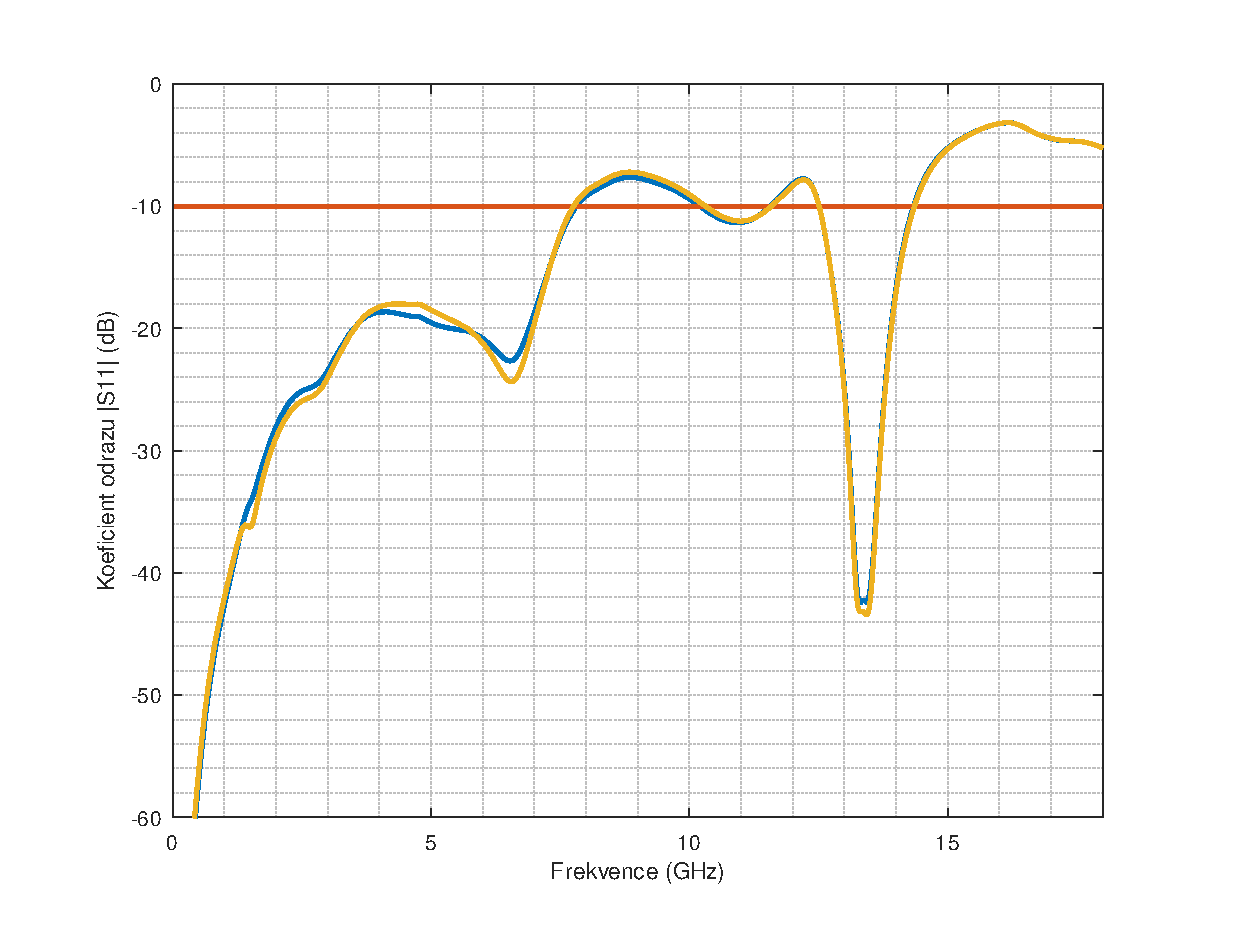
\includegraphics[width=\textwidth,keepaspectratio]{images/measurements/vna_high_low.eps}\caption{Měření vstupní impedance reflektometru pomocí VNA. Modře je označeno měření v logické úrovni 1 a žlutě měření v logické úrovni 0.}\label{vna_impedance}
\end{figure}

\begin{figure}[htbp]
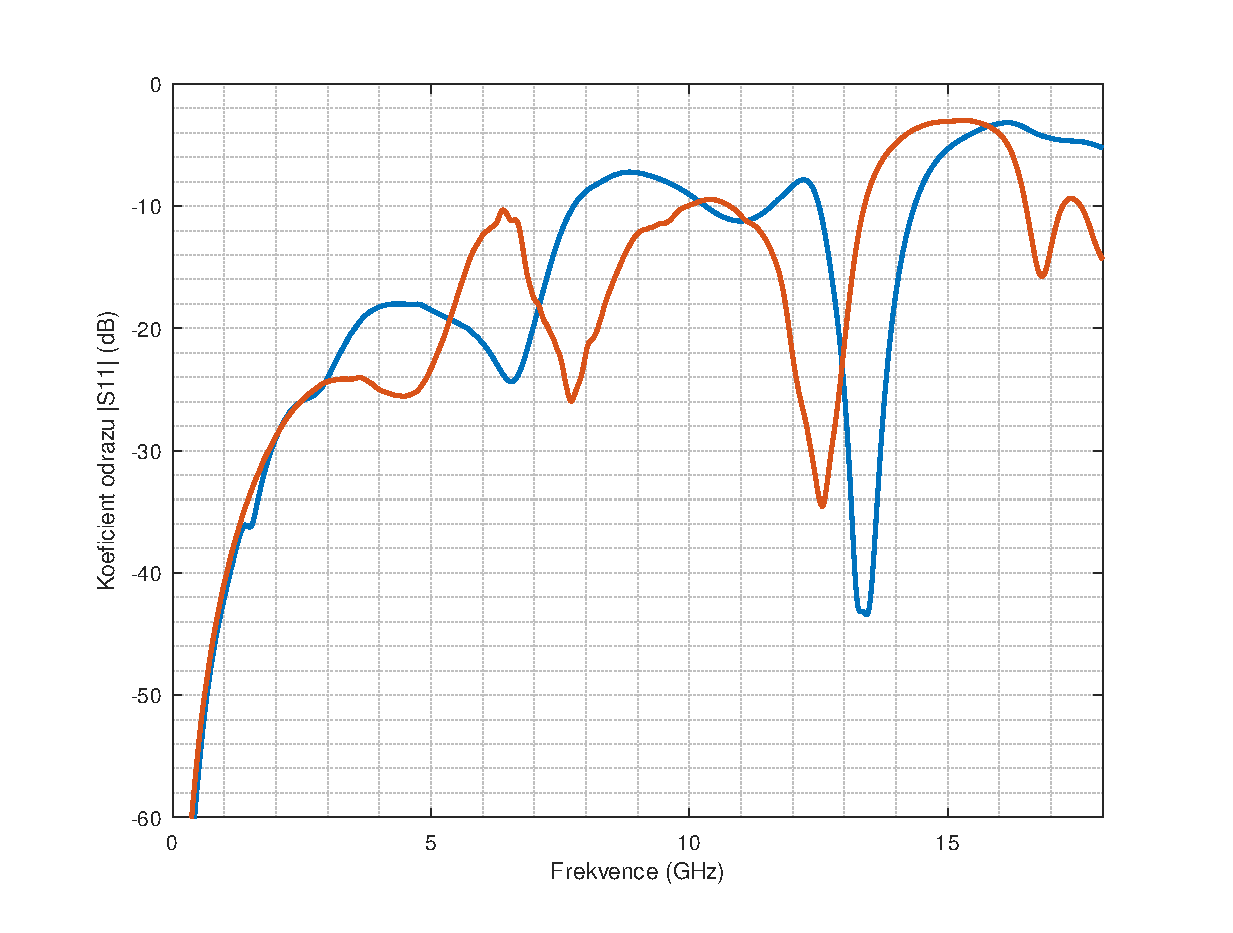
\includegraphics[width=\textwidth,keepaspectratio]{images/measurements/vna_low_blank.eps}\caption{Měření vstupní impedance reflektometru pomocí VNA. Modře je označeno měření v logické úrovni 0, červeně měření na neosazené desce z obr. \ref{pcb_coplanar} terminované \SI{50}{\ohm} terminátorem.}\label{vna_impedance_blank}
\end{figure}

\section{Měření parametrů použitého substrátu}
Pro ověření permitivity použitého substrátu byla vytvořena testovací deska s kalibry pro kalibrační metody \acrshort{TRL} a \acrshort{UOML}. Tato deska je na fotografii \ref{uoml}. Nachází se na ní zeshora postupně kalibrační vedení nulové délky \quotedblbase thru\textquotedblleft , kalibry \quotedblbase short\textquotedblleft , \quotedblbase open\textquotedblleft{} a \quotedblbase match\textquotedblleft{}. Pod nimi se nachází tři vedení různých délek. Zeshora jsou to vedení délek \SI{8}{\milli\meter}, \SI{50}{\milli\meter} a \SI{69.8}{\milli\meter}. Tloušťka substrátu a povrchová úprava je stejná jako u reflektometru, tedy \SI{0.6}{\milli\meter} a olovnatý HAL. Deska byla navržena tak, aby bylo možné na ni namontovat jak kvalitní konektory Southwest Endlaunch, tak i připájet levné konektory použité na reflektometru. Detail kalibru \quotedblbase match\textquotedblleft{} v podobě rezistoru velikosti 0201 je na fotografii \ref{match_detail}, pro srovnání velikosti má otvor napravo od rezistoru průměr \SI{0.3}{\milli\meter}.
\begin{figure}[htbp]
\includegraphics[width=\textwidth,keepaspectratio]{images/measurements/match.jpg}\caption{Detail kalibru \quotedblbase match\textquotedblleft .}\label{match_detail}
\end{figure}

\begin{figure}[htbp]
\includegraphics[width=\textwidth,keepaspectratio]{images/measurements/uoml.jpg}\caption{Testovací deska plošných spojů pro změření parametrů substrátu s připájenými konektory.}\label{uoml}
\end{figure}